\documentclass[border=12pt]{standalone}
\def\pgfsysdriver{pgfsys-dvisvgm.def}
\usepackage[dvisvgm]{xcolor}
\usepackage{xeCJK}
\setCJKmainfont{HaranoAjiGothic-Regular.otf}[BoldFont=HaranoAjiGothic-Bold.otf]
\setCJKsansfont{HaranoAjiGothic-Regular.otf}[BoldFont=HaranoAjiGothic-Bold.otf]
\usepackage{amsmath,amssymb,tikz,lmodern}
\usetikzlibrary{arrows.meta,positioning,calc,fit,backgrounds}
\renewcommand{\familydefault}{\sfdefault}
\definecolor{ink}{HTML}{25322F}
\definecolor{green}{HTML}{246657}
\definecolor{tint}{HTML}{EEF4F0}
\definecolor{soft}{HTML}{C6D2CC}
\definecolor{muted}{HTML}{52615B}
\newif\ifJapanese
\newcommand{\Tx}[2]{\ifJapanese #1\else #2\fi}
\newcommand{\Eff}{\overline{\operatorname{Eff}}}
\newcommand{\heading}[3]{{\color{green}\bfseries #1\quad\Tx{#2}{#3}}\\[5pt]}
% A white rectangle makes the complete citation label clickable, including spaces.
\newcommand{\refurl}[2]{\special{dvisvgm:raw <a xlink:href="#1" target="_blank" rel="noopener noreferrer">}{\setlength{\fboxsep}{0pt}\colorbox{white}{\color{green}\underline{\strut #2}}}\special{dvisvgm:raw </a>}}
\newcommand{\refedge}[3]{\refurl{\csname source#1\endcsname\string##page=#2}{#3}}
\newcommand{\SF}[2]{\refedge{sf}{#1}{#2}}
% GitHub's file preview does not support PDF page fragments.
\newcommand{\LA}[2]{\refurl{\sourcela}{#2}}
\newcommand{\Sch}[2]{\refedge{sch}{#1}{#2}}
\newcommand{\PS}[2]{\refedge{ps}{#1}{#2}}
\tikzset{
 card/.style={draw=soft,fill=white,rounded corners=2pt,align=left,text=ink,font=\fontsize{10.5}{14}\selectfont,inner xsep=12pt,inner ysep=10pt,text width=14.4cm},
 half/.style={card,text width=6.45cm,minimum height=2.05cm},
 result/.style={card,draw=green,fill=tint,line width=.9pt},
 reason/.style={align=left,text=muted,font=\fontsize{9}{12}\selectfont,inner sep=0pt,text width=12.7cm},
 branchreason/.style={reason,text width=5.95cm},
 edge/.style={-{Stealth[length=2.4mm]},draw=green,line width=1pt},
 wire/.style={draw=green,line width=1pt},
}
% Keep the arrow in a dedicated left gutter; explanations never cover it.
\newcommand{\flow}[3]{
 \coordinate (#2-from) at ($(#1.south)+(-6.9,0)$);
 \coordinate (#2-to) at ($(#2.north)+(-6.9,0)$);
 \draw[edge] (#2-from)--(#2-to);
 \node[reason,anchor=west] (#2-reason) at ($(#2-from)!.5!(#2-to)+(.55,0)$) {#3};
}


\newcommand{\CiteSource}[2]{\refurl{\csname source#1\endcsname}{#2}}

\expandafter\def\csname sourceU\endcsname{https://github.com/openai/math/blob/adc7f1241b42e322a6451854ab7e4b4c146bf78a/preprints/Uniform-Pluricanonical-Iitaka-Fibrations-October-3-2026/paper.pdf}
\expandafter\def\csname sourceLA\endcsname{https://github.com/openai/math/blob/adc7f1241b42e322a6451854ab7e4b4c146bf78a/preprints/Log-abundance-in-characteristic-zero-September-24-2026/paper.pdf}
\expandafter\def\csname sourceSD\endcsname{https://github.com/openai/math/blob/adc7f1241b42e322a6451854ab7e4b4c146bf78a/preprints/Arithmetic-Stein-degree-bounds-for-log-Calabi-Yau-pairs-September-25-2026/paper.pdf}
\expandafter\def\csname sourceUfour\endcsname{https://github.com/openai/math/blob/adc7f1241b42e322a6451854ab7e4b4c146bf78a/preprints/Uniform-effective-log-Iitaka-fibrations-for-fourfolds-September-26-2026/paper.pdf}
\expandafter\def\csname sourceR\endcsname{https://github.com/openai/math/blob/adc7f1241b42e322a6451854ab7e4b4c146bf78a/preprints/Relative-denominators-and-effective-systems-for-log-Calabi-Yau-fibrations-September-27-2026/paper.pdf}
\expandafter\def\csname sourceLog\endcsname{https://github.com/openai/math/blob/adc7f1241b42e322a6451854ab7e4b4c146bf78a/preprints/Uniform-log-Iitaka-fibrations-and-bounded-moduli-denominators-October-4-2026/uniform-log-iitaka.pdf}
\expandafter\def\csname sourceSLC\endcsname{https://github.com/openai/math/blob/adc7f1241b42e322a6451854ab7e4b4c146bf78a/preprints/Uniform-indices-for-semi-log-canonical-log-Calabi-Yau-pairs-October-5-2026/uniform-slc-index.pdf}
\expandafter\def\csname sourceBZ\endcsname{https://arxiv.org/pdf/1410.0938v2}

\Japanesetrue
\begin{document}
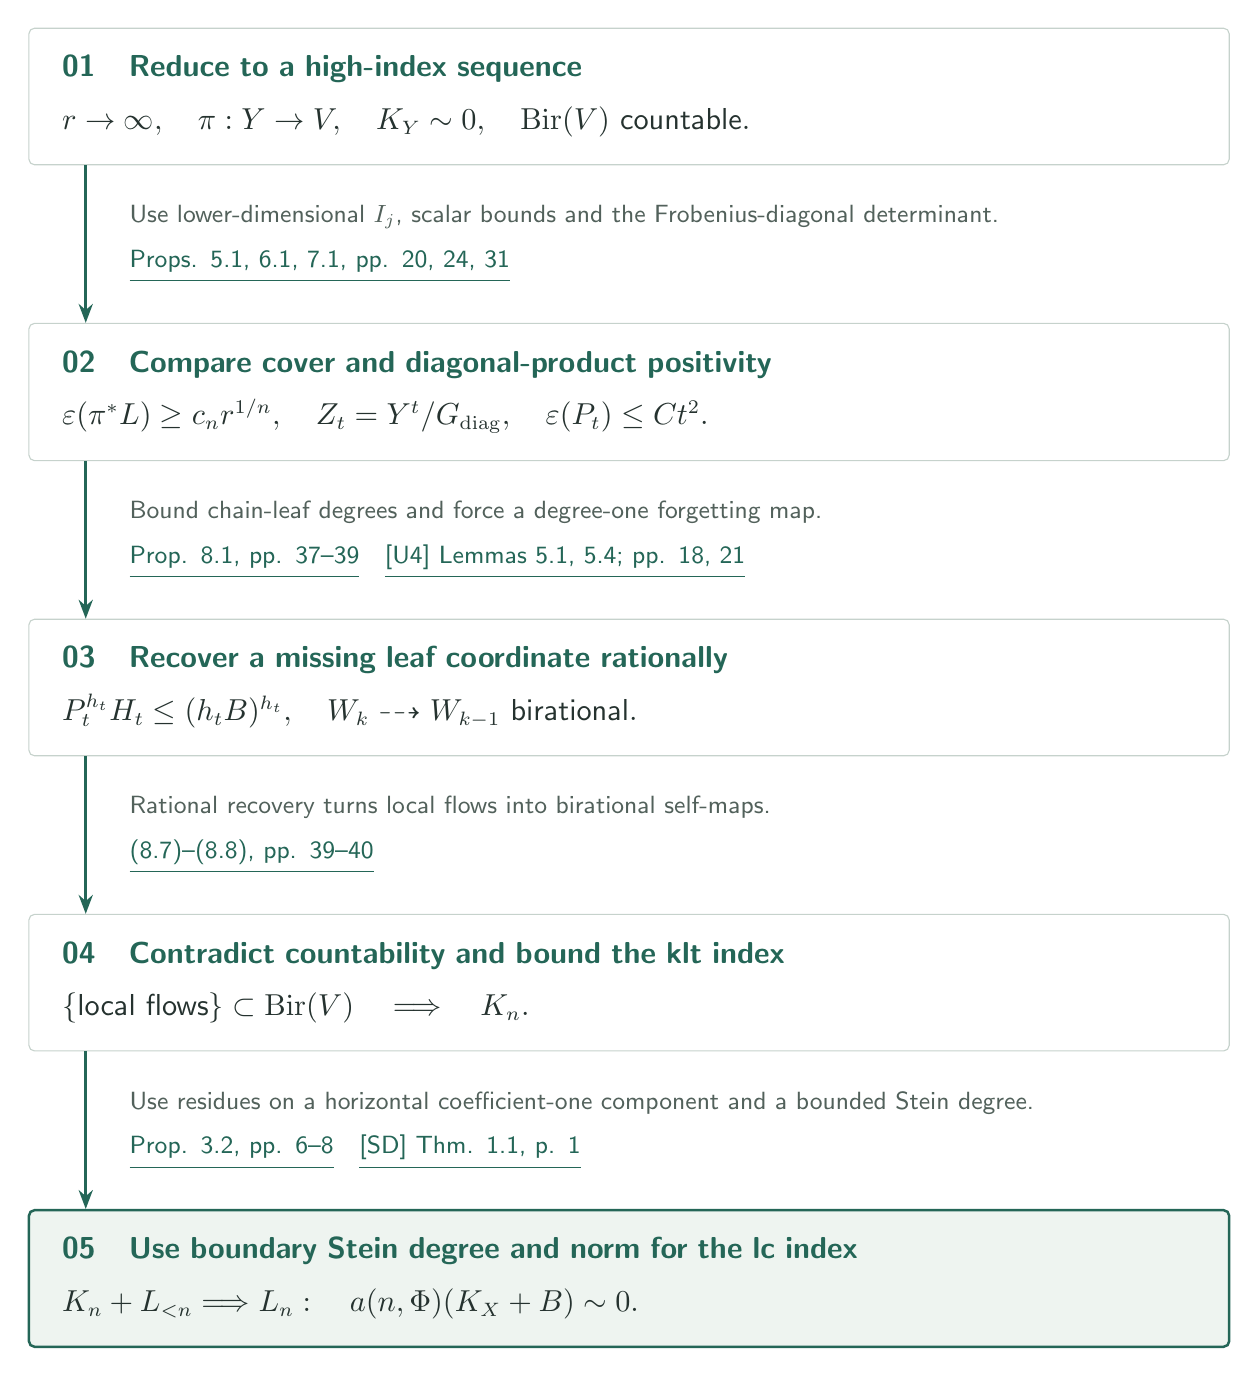
\begin{tikzpicture}
\node[card] (n0) {\heading{01}{高指数列に帰着する}{Reduce to a high-index sequence}$r\to\infty,\quad\pi:Y\to V,\quad K_Y\sim0,\quad\operatorname{Bir}(V)\ \text{countable}.$};
\node[card,below=2.0cm of n0] (n1) {\heading{02}{被覆と対角積に反対向きの評価を得る}{Compare cover and diagonal-product positivity}$\varepsilon(\pi^*L)\ge c_nr^{1/n},\quad Z_t=Y^t/G_{\rm diag},\quad\varepsilon(P_t)\le Ct^2.$};
\flow{n0}{n1}{\Tx{低次元 $I_j$ の scalar 評価と Frobenius 対角の行列式を使う。}{Use lower-dimensional $I_j$, scalar bounds and the Frobenius-diagonal determinant.}\\[4pt]\CiteSource{U}{Props. 5.1, 6.1, 7.1, pp. 20, 24, 31}}
\node[card,below=2.0cm of n1] (n2) {\heading{03}{葉の座標を有理的に回収する}{Recover a missing leaf coordinate rationally}$P_t^{h_t}H_t\le(h_tB)^{h_t},\quad W_k\dashrightarrow W_{k-1}\ \text{birational}.$};
\flow{n1}{n2}{\Tx{鎖の葉の次数を抑え、座標忘却の次数1を強制する。}{Bound chain-leaf degrees and force a degree-one forgetting map.}\\[4pt]\CiteSource{U}{Prop. 8.1, pp. 37--39}\quad \CiteSource{Ufour}{[U4] Lemmas 5.1, 5.4; pp. 18, 21}}
\node[card,below=2.0cm of n2] (n3) {\heading{04}{可算性との矛盾から零境界指数へ}{Contradict countability and bound the klt index}$\{\text{local flows}\}\subset\operatorname{Bir}(V)\quad\Longrightarrow\quad K_n.$};
\flow{n2}{n3}{\Tx{有理的な座標回収で局所 flow を双有理写像にする。}{Rational recovery turns local flows into birational self-maps.}\\[4pt]\CiteSource{U}{(8.7)--(8.8), pp. 39--40}}
\node[result,below=2.0cm of n3] (n4) {\heading{05}{境界の Stein 次数と norm で lc 指数へ}{Use boundary Stein degree and norm for the lc index}$K_n+L_{<n}\Longrightarrow L_n:\quad a(n,\Phi)(K_X+B)\sim0.$};
\flow{n3}{n4}{\Tx{水平な係数1成分の留数と有界な Stein 次数を使う。}{Use residues on a horizontal coefficient-one component and a bounded Stein degree.}\\[4pt]\CiteSource{U}{Prop. 3.2, pp. 6--8}\quad \CiteSource{SD}{[SD] Thm. 1.1, p. 1}}
\end{tikzpicture}
\end{document}
